\documentclass[11pt,a4paper]{article}

% ---------------------------------------------------------------- packages
\usepackage[a4paper,top=2.6cm,bottom=2.8cm,left=2.4cm,right=2.4cm]{geometry}
\usepackage{fontspec}
\setmainfont{Georgia}
\newfontfamily\headingfont{Century Gothic}
\usepackage[table]{xcolor}
\usepackage{tikz}
\usetikzlibrary{arrows.meta,positioning,shapes.geometric,fit,backgrounds,calc}
\usepackage{fancyhdr}
\usepackage{titlesec}
\usepackage[most]{tcolorbox}
\usepackage{listings}
\usepackage{booktabs}
\usepackage{longtable}
\usepackage{array}
\usepackage{enumitem}
\usepackage{hyperref}
\usepackage{tabularx}
\usepackage{multirow}
\usepackage{needspace}

% ---------------------------------------------------------------- palette
\definecolor{navy}{HTML}{15224A}
\definecolor{deepnavy}{HTML}{0B1330}
\definecolor{teal}{HTML}{0FA3A3}
\definecolor{tealbright}{HTML}{1FD1C1}
\definecolor{amber}{HTML}{E8A33D}
\definecolor{coral}{HTML}{E8604C}
\definecolor{slate}{HTML}{5B6B87}
\definecolor{paper}{HTML}{FBFBFD}
\definecolor{cardbg}{HTML}{F3F5FA}
\definecolor{inkgray}{HTML}{2A2F3B}

\pagecolor{paper}
\color{inkgray}

% ---------------------------------------------------------------- headings
\titleformat{\section}
  {\headingfont\Large\bfseries\color{navy}}
  {\thesection}{0.5em}{}
  [\vspace{-0.3em}{\color{teal}\rule{\linewidth}{1.4pt}}]
\titlespacing{\section}{0pt}{1.6em}{0.9em}

\titleformat{\subsection}
  {\headingfont\large\bfseries\color{navy}}
  {\thesubsection}{0.5em}{}
\titlespacing{\subsection}{0pt}{1.3em}{0.5em}

\titleformat{\subsubsection}
  {\headingfont\normalsize\bfseries\color{teal}}
  {\thesubsubsection}{0.5em}{}
\titlespacing{\subsubsection}{0pt}{1em}{0.3em}

% ---------------------------------------------------------------- header/footer
\pagestyle{fancy}
\fancyhf{}
\renewcommand{\headrulewidth}{0pt}
\renewcommand{\footrulewidth}{0.4pt}
\fancyfoot[L]{\small\color{slate}\headingfont Agentic PIEAS ERP Synchronization}
\fancyfoot[R]{\small\color{slate}\headingfont\thepage}
\fancypagestyle{plain}{
  \fancyhf{}
  \renewcommand{\headrulewidth}{0pt}
  \renewcommand{\footrulewidth}{0pt}
}

% ---------------------------------------------------------------- misc
\setlist[itemize]{leftmargin=1.3em,itemsep=0.25em,topsep=0.3em}
\setlist[enumerate]{leftmargin=1.5em,itemsep=0.3em,topsep=0.3em}
\renewcommand{\arraystretch}{1.25}
\sloppy
\emergencystretch=2.5em
\hbadness=3000
\hfuzz=2pt

\hypersetup{
  colorlinks=true,
  linkcolor=teal,
  urlcolor=teal,
  citecolor=teal,
  pdftitle={Agentic PIEAS ERP Synchronization},
  pdfauthor={PIEAS},
  pdfsubject={Multi-Agent LangGraph ETL System},
}

\lstdefinestyle{code}{
  backgroundcolor=\color{cardbg},
  basicstyle=\ttfamily\small\color{inkgray},
  keywordstyle=\color{teal}\bfseries,
  commentstyle=\color{slate}\itshape,
  stringstyle=\color{amber},
  numberstyle=\tiny\color{slate},
  frame=single,
  rulecolor=\color{slate!40},
  framesep=6pt,
  xleftmargin=8pt,
  xrightmargin=8pt,
  breaklines=true,
  showstringspaces=false,
  tabsize=2,
}
\lstset{style=code}

% callout boxes
\newtcolorbox{principlebox}[1]{
  enhanced, breakable,
  colback=cardbg, colframe=teal, boxrule=0pt,
  leftrule=3.2pt, sharp corners, top=8pt, bottom=8pt,
  left=12pt, right=12pt,
  title={#1}, coltitle=navy, fonttitle=\headingfont\bfseries,
  attach boxed title to top left={xshift=0mm,yshift*=-\tcboxedtitleheight/2},
  boxed title style={colback=paper, boxrule=0pt},
}
\newtcolorbox{warnbox}[1]{
  enhanced, breakable,
  colback=coral!8, colframe=coral, boxrule=0pt,
  leftrule=3.2pt, sharp corners, top=8pt, bottom=8pt,
  left=12pt, right=12pt,
  title={#1}, coltitle=coral!55!black, fonttitle=\headingfont\bfseries,
  attach boxed title to top left={xshift=0mm,yshift*=-\tcboxedtitleheight/2},
  boxed title style={colback=paper, boxrule=0pt},
}
\newtcolorbox{fixbox}[1]{
  enhanced, breakable,
  colback=teal!6, colframe=teal, boxrule=0pt,
  leftrule=3.2pt, sharp corners, top=8pt, bottom=8pt,
  left=12pt, right=12pt,
  title={#1}, coltitle=navy, fonttitle=\headingfont\bfseries,
  attach boxed title to top left={xshift=0mm,yshift*=-\tcboxedtitleheight/2},
  boxed title style={colback=paper, boxrule=0pt},
}
% A challenge and its resolution as one unbreakable card (upper/lower split via
% \tcblower), so the pair always moves to the next page together rather than
% splitting and leaving an orphaned fragment.
\newtcolorbox{challengebox}[1]{
  enhanced, sharp corners, boxrule=0pt,
  colback=cardbg, coltext=inkgray,
  leftrule=3.2pt, colframe=coral,
  top=9pt, bottom=9pt, left=13pt, right=13pt,
  title={#1}, coltitle=coral!50!black, fonttitle=\headingfont\bfseries\small,
  attach boxed title to top left={xshift=0mm,yshift*=-\tcboxedtitleheight/2},
  boxed title style={colback=paper, boxrule=0pt},
  before lower={\par\vspace{5pt}{\color{teal!45!black}\hrule height 0.6pt}\vspace{7pt}{\headingfont\bfseries\small\color{teal!55!black}Resolution\ \ }},
}

\begin{document}

% ================================================================ TITLE PAGE
\begin{titlepage}
\newgeometry{margin=0cm}
\pagecolor{deepnavy}

\begin{tikzpicture}[remember picture,overlay,shift={(current page.south west)}]
  \fill[deepnavy] (0,0) rectangle (21,29.7);

  % faint grid motif
  \begin{scope}[opacity=0.10]
    \foreach \x in {0,1,...,21}{\draw[teal] (\x,0) -- (\x,29.7);}
    \foreach \y in {0,1,...,29}{\draw[teal] (0,\y) -- (21,\y);}
  \end{scope}

  % glow accent circles
  \fill[tealbright,opacity=0.08] (18.5,25) circle (5.2);
  \fill[teal,opacity=0.10] (2,4) circle (4.4);

  % top accent bar
  \fill[teal] (0,29.7) rectangle (21,29.4);

  % pipeline glyph motif: a small decorative logo, clear of all text, top-right
  \begin{scope}[shift={(14.7,26.3)}]
    \draw[teal, line width=0.9pt] (0.72,0) -- (1.48,0);
    \draw[teal, line width=0.9pt] (2.23,0) -- (2.98,0);
    \draw[teal, line width=0.9pt] (3.73,0) -- (4.48,0);
    \node[draw=tealbright,line width=1.1pt,circle,minimum size=1.3cm,fill=deepnavy] (o) at (0,0) {\color{tealbright}\headingfont\footnotesize\bfseries O};
    \node[draw=teal,line width=1pt,circle,minimum size=1.1cm,fill=deepnavy] (e) at (1.85,0) {\color{teal}\headingfont\scriptsize\bfseries E};
    \node[draw=amber,line width=1pt,circle,minimum size=1.1cm,fill=deepnavy] (t) at (3.6,0) {\color{amber}\headingfont\scriptsize\bfseries T};
    \node[draw=coral,line width=1pt,circle,minimum size=1.1cm,fill=deepnavy] (l) at (5.35,0) {\color{coral}\headingfont\scriptsize\bfseries L};
  \end{scope}

  % left-aligned title column -- each block anchored to the previous one's
  % actual rendered edge, so spacing stays correct regardless of font metrics.
  % Anchored around the page's vertical middle for a balanced, uncrowded page.
  \node[anchor=north west, text width=16cm] (inst) at (2.4,18.6)
    {\color{teal}\headingfont\footnotesize\bfseries PAKISTAN INSTITUTE OF ENGINEERING AND APPLIED SCIENCES};

  \node[anchor=north west, text width=16.3cm, yshift=-0.55cm] (title) at (inst.south west)
    {\color{white}\headingfont\bfseries\fontsize{34}{41}\selectfont Agentic PIEAS ERP\\[0.1em] Synchronization};

  \node[anchor=north west, text width=16cm, yshift=-0.6cm] (sub) at (title.south west)
    {\color{tealbright!85!white}\headingfont\fontsize{15}{20}\selectfont A Four-Agent LangGraph System for Continuous, Unattended Data Migration into OpenEduCat};

  \draw[teal!55,line width=0.8pt] ($(sub.south west)+(0,-0.55)$) -- ($(sub.south west)+(14,-0.55)$);

  \node[anchor=north west, text width=14cm, yshift=-1.1cm] (desc) at (sub.south west)
    {\color{white!85!black}\headingfont\footnotesize
     A legacy learning-management system, with no API and no webhooks, kept in
     perpetual synchrony with a modern Odoo-based ERP --- through bulk migration,
     incremental updates, and unattended deletion detection.};

  % faint horizontal rule + tagline anchored to the bottom band, balancing
  % the lower half of the page against the text block above
  \node[anchor=south west, text width=16cm] (tag) at (2.4,5.1)
    {\color{slate!70!white}\headingfont\itshape\footnotesize Specialized agents. Strict state control. Complete data integrity.};

  % bottom credential strip
  \fill[teal] (0,0) rectangle (21,3.6);
  \fill[deepnavy,opacity=0.12] (0,0) rectangle (21,3.6);
  \node[align=left,text width=6.2cm] at (3.6,2.5) {\color{deepnavy}\headingfont\bfseries\footnotesize PROJECT TYPE\\[3pt]\color{deepnavy}\footnotesize\fontsize{9}{11}\selectfont Internship / Systems Integration};
  \node[align=left,text width=6.2cm] at (10.5,2.5) {\color{deepnavy}\headingfont\bfseries\footnotesize STACK\\[3pt]\color{deepnavy}\footnotesize\fontsize{9}{11}\selectfont LangGraph \textbullet\ Gemini \textbullet\ MySQL \textbullet\ Odoo XML-RPC};
  \node[align=left,text width=6.2cm] at (17.4,2.5) {\color{deepnavy}\headingfont\bfseries\footnotesize DATE\\[3pt]\color{deepnavy}\footnotesize\fontsize{9}{11}\selectfont August 2026};
\end{tikzpicture}
\end{titlepage}
\restoregeometry
\pagecolor{paper}
\color{inkgray}

% ================================================================ ABSTRACT
\thispagestyle{plain}
\vspace*{0.5em}
\begin{center}
{\headingfont\Large\bfseries\color{navy} Abstract}
\end{center}
\vspace{0.6em}
\begin{tcolorbox}[enhanced,colback=cardbg,colframe=navy,boxrule=0.6pt,sharp corners,left=16pt,right=16pt,top=12pt,bottom=12pt]
The PIEAS Learning Management System is a legacy application with no external API, no webhook mechanism, and no capacity to announce its own state changes. Migrating its data into a modern OpenEduCat (Odoo) Education ERP therefore requires the \emph{target} system to actively discover changes at the source, rather than being notified of them. This report documents the design, implementation, and verification of a four-agent synchronization system built on LangGraph, in which a single \textbf{Orchestrator} agent owns all state and scheduling decisions, and three stateless workers --- \textbf{Extractor}, \textbf{Transformer}, and \textbf{Loader} --- execute exactly what they are instructed to, nothing more. The same pipeline drives three operational phases: an initial bulk migration, a recurring incremental synchronization driven by a strictly advancing timestamp watermark, and a slower deletion scan that detects records absent from the source via an in-memory set difference. Large-language-model reasoning (Google Gemini) is applied sparingly and cached aggressively --- once per table for schema mapping, once per query shape for SQL generation --- so that per-row execution remains deterministic, fast, and reproducible even across thousands of records. The system was implemented and verified end-to-end against a live MySQL source and a live Odoo 19 instance, migrating 99 records across eight related entities with zero data loss, correctly routing examination data into OpenEduCat's Examination module, and correctly distinguishing an archivable deletion from a destructive one.
\end{tcolorbox}

\vspace{1.4em}
{\headingfont\bfseries\color{navy}\normalsize Keywords} --- multi-agent systems, LangGraph, ERP data migration, Odoo, OpenEduCat, incremental synchronization, watermarking, large language models, XML-RPC.

\vspace{2.2em}
\tableofcontents

\newpage

% ================================================================ 1. INTRO
\section{Introduction}

\subsection{Problem Statement}
The Pakistan Institute of Engineering and Applied Sciences (PIEAS) operates a custom-built, standalone Learning Management System (LMS) that has accumulated years of institutional data: departments, courses, batches, subjects, faculty, students, examinations, and results. The institute is migrating academic records management to \textbf{OpenEduCat}, an open-source Education ERP built on the Odoo framework, to eliminate data silos and reduce the maintenance burden of a bespoke system.

This upgrade introduces a severe technical constraint: \textbf{the source system is completely silent}. The legacy PIEAS LMS exposes no API, issues no webhooks, and has no mechanism to push a notification when a row is inserted, updated, or deleted. Any synchronization strategy must therefore treat the source purely as a passive, query-only surface --- OpenEduCat must actively \emph{hunt} for what has changed.

This asymmetry is the central design problem addressed by this report:
\begin{center}
\textit{``How do you synchronize a system that cannot tell you when its data changes?''}
\end{center}

\subsection{Design Constraints}
Four constraints shaped every subsequent decision:
\begin{enumerate}
  \item \textbf{Zero modification of the legacy source.} The PIEAS LMS schema, application, and data cannot be altered. No trigger, no dirty-flag column, no outbox table may be added to it.
  \item \textbf{No notification channel.} Change detection must be pull-based, driven entirely from the target side.
  \item \textbf{Correctness under partial failure.} A crashed or interrupted sync run must never silently lose a change or duplicate a record.
  \item \textbf{Respect for the target's business rules.} Writes into Odoo must go through its Object-Relational Mapping (ORM) layer so that computed fields, validation, and related-record bookkeeping are honoured --- not bypassed.
\end{enumerate}

\subsection{Solution Overview}
The system implements a specialized four-agent architecture, orchestrated with \textbf{LangGraph}, in which exactly one agent is permitted to make decisions and hold memory, while three others are strictly stateless executors. The same pipeline structure serves three distinct operational phases --- bulk migration, incremental synchronization, and deletion detection --- without any change to the workers' logic, differing only in the instructions the Orchestrator issues. Large language model reasoning (Gemini) is used for schema understanding and query authorship, not for per-record decision making, keeping the system both intelligent and fast.

\newpage
% ================================================================ 2. ARCHITECTURE
\section{System Architecture}

\subsection{Design Principle: One Agent, One Job}
Rather than a monolithic script, the solution is built as a four-agent ecosystem governed by a strict separation of concerns: a single agent decides, three agents execute.

\begin{center}
\resizebox{\textwidth}{!}{%
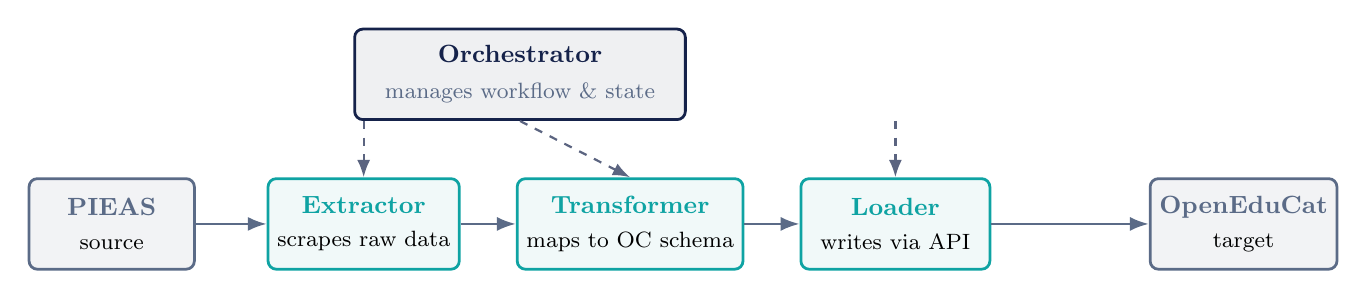
\begin{tikzpicture}[
    node distance=1.1cm and 1.3cm,
    font=\headingfont\small,
    every node/.style={align=center},
    box/.style={draw, rounded corners=3pt, minimum height=1.15cm, minimum width=2.4cm, line width=1pt, fill=cardbg},
    orch/.style={box, draw=navy, fill=navy!7, minimum width=4.2cm},
    work/.style={box, draw=teal, fill=teal!6},
    ext/.style={box, draw=tealbright, fill=tealbright!10},
    src/.style={box, draw=slate, fill=slate!8, minimum width=2.1cm},
    arr/.style={-{Latex[length=2.4mm]}, line width=0.9pt, color=slate},
    darr/.style={-{Latex[length=2.2mm]}, line width=0.8pt, dashed, color=navy!70},
  ]
  \node[orch] (orch) {\color{navy}\bfseries Orchestrator\\[2pt]\footnotesize\color{slate} manages workflow \& state};
  \node[src, left=2.0cm of orch, yshift=-1.9cm] (pieas) {\color{slate}\bfseries PIEAS\\[1pt]\footnotesize source};
  \node[work, right=0.9cm of pieas, yshift=0] (extractor) {\color{teal}\bfseries Extractor\\[1pt]\footnotesize scrapes raw data};
  \node[work, right=0.7cm of extractor] (transformer) {\color{teal}\bfseries Transformer\\[1pt]\footnotesize maps to OC schema};
  \node[work, right=0.7cm of transformer] (loader) {\color{teal}\bfseries Loader\\[1pt]\footnotesize writes via API};
  \node[src, right=2.0cm of loader] (odoo) {\color{slate}\bfseries OpenEduCat\\[1pt]\footnotesize target};

  \draw[arr] (pieas) -- (extractor);
  \draw[arr] (extractor) -- (transformer);
  \draw[arr] (transformer) -- (loader);
  \draw[arr] (loader) -- (odoo);

  \draw[darr] (orch.south -| extractor) -- (extractor.north);
  \draw[darr] (orch.south) -- (transformer.north);
  \draw[darr] (orch.south -| loader) -- (loader.north);
\end{tikzpicture}%
}
\end{center}

\subsection{Agent Responsibilities}

\begin{longtable}{@{}>{\raggedright\arraybackslash}p{2.7cm}>{\raggedright\arraybackslash}p{2.1cm}>{\raggedright\arraybackslash}p{8.6cm}@{}}
\toprule
\rowcolor{navy!10}
\textbf{\color{navy}Agent} & \textbf{\color{navy}Holds State} & \textbf{\color{navy}Role} \\
\midrule
\endhead
\textbf{Orchestrator} & \color{teal!70!black}\bfseries Yes --- exclusively &
The only decision-maker in the system. Reads the state store to determine each entity's phase (bulk vs.\ incremental), writes natural-language extraction instructions, evaluates fetched rows against its memory of prior syncs, and is the sole agent permitted to advance the synchronization watermark. \\
\addlinespace
\textbf{Extractor} & No &
The pure fetcher, and the \emph{only} agent that ever touches PIEAS. Takes an instruction, authors (or reuses cached) read-only SQL, and returns raw rows. Performs no comparisons and makes no decisions. \\
\addlinespace
\textbf{Transformer} & No &
A pure function. Maps the PIEAS relational schema onto OpenEduCat's Odoo models using a cached, per-entity mapping plan. Identical logic executes regardless of which phase invoked it. \\
\addlinespace
\textbf{Loader} & No &
The writer. Executes the final action against Odoo over XML-RPC: create, update, or archive. On rejection, consults the Orchestrator's diagnostic reasoning to decide whether to retry, repair, or quarantine the record. \\
\bottomrule
\end{longtable}

\subsection{The Orchestrator's Control Loop}
Each synchronization run advances through a four-step cycle, repeated once per configured entity:

\begin{center}
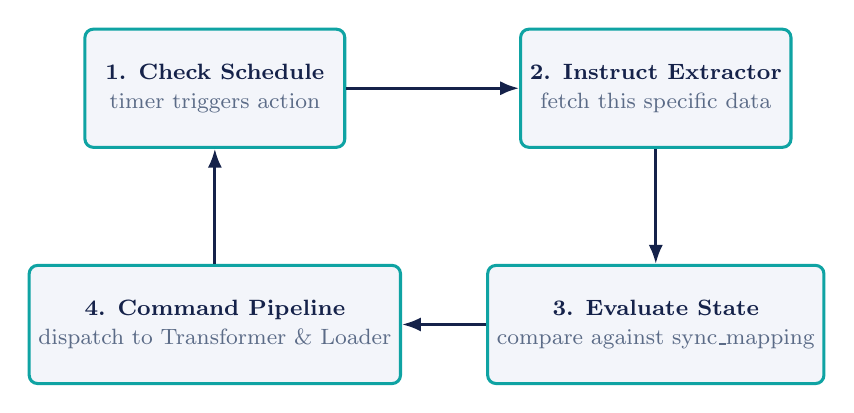
\begin{tikzpicture}[
    font=\headingfont\footnotesize,
    node distance=2.5cm,
    every node/.style={align=center},
    stepbox/.style={draw=teal, line width=1.1pt, rounded corners=3pt, fill=cardbg, minimum width=3.3cm, minimum height=1.5cm},
    arr/.style={-{Latex[length=2.4mm]}, line width=1pt, color=navy},
  ]
  \node[stepbox] (s1) at (0,0) {\color{navy}\bfseries 1. Check Schedule\\[1pt]\footnotesize\color{slate} timer triggers action};
  \node[stepbox] (s2) at (5.6,0) {\color{navy}\bfseries 2. Instruct Extractor\\[1pt]\footnotesize\color{slate} fetch this specific data};
  \node[stepbox] (s3) at (5.6,-3.0) {\color{navy}\bfseries 3. Evaluate State\\[1pt]\footnotesize\color{slate} compare against sync\_mapping};
  \node[stepbox] (s4) at (0,-3.0) {\color{navy}\bfseries 4. Command Pipeline\\[1pt]\footnotesize\color{slate} dispatch to Transformer \& Loader};

  \draw[arr] (s1) -- (s2);
  \draw[arr] (s2) -- (s3);
  \draw[arr] (s3) -- (s4);
  \draw[arr] (s4) -- (s1);
\end{tikzpicture}
\end{center}

The Orchestrator's memory, the \texttt{sync\_mapping} table, bridges every PIEAS primary key to its corresponding Odoo record ID, and is the single source of truth consulted at step 3.

\newpage
% ================================================================ 3. PHASES
\section{Operational Phases}

A single pipeline drives three phases; only the instruction issued by the Orchestrator differs.

\begin{table}[h]
\centering
\begin{tabularx}{\textwidth}{@{}l>{\raggedright\arraybackslash}X>{\raggedright\arraybackslash}X>{\raggedright\arraybackslash}X@{}}
\toprule
\rowcolor{navy!10}
\textbf{\color{navy}Phase} & \textbf{\color{navy}Trigger} & \textbf{\color{navy}Extractor Instruction} & \textbf{\color{navy}Loader Operation} \\
\midrule
\textbf{1. Bulk Migration} & State store is empty & Fetch every row, paginating until exhausted & Predominantly \texttt{create} \\
\textbf{2. Incremental (Fast Pulse)} & Timer, every $N$ minutes & \texttt{WHERE last\_updated > watermark} & \texttt{upsert} \\
\textbf{3. Deletion Scan (Slow Pulse)} & Timer, once daily & Fetch the \texttt{id} column of every current row & \texttt{archive} \\
\bottomrule
\end{tabularx}
\end{table}

\subsection{Why Two Distinct Rhythms}
Because PIEAS cannot push notifications, the Orchestrator must actively hunt for two structurally different kinds of change, and a single polling strategy cannot catch both.

\begin{principlebox}{The Fast Pulse --- Timestamp Watermarks}
Every source table carries a \texttt{last\_updated} column, maintained automatically by MySQL (\texttt{ON UPDATE CURRENT\_TIMESTAMP}). The Orchestrator records a \texttt{last\_synced\_at} watermark per entity and instructs the Extractor to fetch only rows strictly newer than it. After a successful load, the watermark advances to the newest timestamp seen --- and \emph{only} then, so a partially-failed batch is safely retried on the next tick rather than silently skipped.

\textbf{Anti-pattern, deliberately avoided:} a boolean \texttt{sync\_pending} flag. If a row changes again while it is mid-sync, naively resetting the flag to \texttt{0} after the first sync silently drops the second change. A monotonically advancing timestamp cannot lose a write in this way.
\end{principlebox}

\begin{principlebox}{The Slow Pulse --- Ghost Detection via Set Difference}
A \texttt{WHERE last\_updated > watermark} query is structurally incapable of finding a row that no longer exists --- there is nothing left to query. Deletion detection is therefore a different operation entirely: the Extractor pulls \emph{only} the current list of primary keys from PIEAS, and the Orchestrator computes the set difference against the primary keys it remembers as active in \texttt{sync\_mapping}. Anything present in memory but absent from the fresh fetch is a \emph{ghost} --- conceptually equivalent to:
\begin{lstlisting}[language=SQL]
SELECT m.pieas_id FROM sync_mapping m
LEFT JOIN pieas_table s ON s.id = m.pieas_id
WHERE s.id IS NULL AND m.status = 'active'
\end{lstlisting}
This scan is heavier than the fast pulse (it must enumerate every live ID) but far cheaper than re-fetching every column, so it is scheduled far less frequently.
\end{principlebox}

\subsection{Archiving, Not Destroying}
When the slow pulse confirms a deletion, the Loader does not delete the corresponding Odoo record. It sets \texttt{active = False} wherever the target model supports it.

\begin{principlebox}{Why Archive}
\begin{itemize}
  \item \textbf{Historical integrity.} Deleting a student record would cascade into --- or orphan --- their grade history and past enrolments. An archived record preserves the full academic trail.
  \item \textbf{Reversibility.} A PIEAS-side rename or a temporary status toggle can look identical to a deletion from the outside. Archiving is safely undone: if the record reappears on a later fetch, the next incremental sync simply un-archives it.
  \item \textbf{Model-aware fallback.} Not every Odoo model exposes an \texttt{active} field --- line-item models such as \texttt{op.exam.attendees} have none. The Loader inspects the live schema at runtime and falls back to a true removal only when no archived state exists to move the record into.
\end{itemize}
\end{principlebox}

\newpage
% ================================================================ 4. LLM STRATEGY
\section{Large-Language-Model Strategy}

\subsection{Reasoning Once, Executing Deterministically}
A naive design might invoke an LLM for every single record synchronized. This was deliberately rejected: it is slow, expensive, non-deterministic across runs, and unnecessary. Gemini is instead used to reason about \emph{shape} --- schemas, mappings, and query structure --- exactly once per distinct need, with the result cached to disk. Per-row execution then runs as ordinary, deterministic Python driven by that cached plan.

\begin{table}[h]
\centering
\begin{tabularx}{\textwidth}{@{}l>{\raggedright\arraybackslash}X l@{}}
\toprule
\rowcolor{navy!10}
\textbf{\color{navy}Agent} & \textbf{\color{navy}What Gemini Is Asked} & \textbf{\color{navy}Frequency} \\
\midrule
Orchestrator & Plan each entity's phase and author the Extractor's natural-language instruction & Once per run \\
Extractor & Translate the instruction into a single, validated \texttt{SELECT} statement & Once per (entity, phase) --- \emph{cached} \\
Transformer & Map MySQL columns onto Odoo's live \texttt{fields\_get()} response & Once per entity --- \emph{cached} \\
Loader & Triage a rejected write and choose a recovery action & Once per distinct error signature \\
\bottomrule
\end{tabularx}
\end{table}

As a direct consequence, a bulk migration of thousands of rows costs on the order of a dozen model calls, not thousands, and produces identical output on every re-run --- an essential property for a system that must be demonstrably reliable, not merely occasionally correct.

\subsection{The Model Proposes; the Live Schema Decides}
Every artifact an LLM produces is treated as an untrusted proposal and passed through a deterministic sanitizer before it is used:

\begin{itemize}
  \item Generated SQL must parse as exactly one \texttt{SELECT} statement, reference only a whitelisted table, and use exactly the expected number of bind parameters --- otherwise it is rejected outright and a hand-written default query is used instead.
  \item Mapping plans are filtered against Odoo's live \texttt{fields\_get()} response. Any field the model names that is not writable --- notably \textbf{readonly, related-and-stored} fields such as \texttt{op.exam.course\_id}, which Odoo derives automatically from \texttt{session\_id} --- is silently dropped before it can cause a write failure.
  \item Foreign keys the model overlooks are recovered independently from MySQL's \texttt{information\_schema}, so relational correctness never depends solely on the model noticing a key.
  \item If Gemini is unreachable or its daily free-tier quota is exhausted, every agent falls back to a deterministic plan, and the synchronization run completes rather than halting.
\end{itemize}

\newpage
% ================================================================ 5. IMPLEMENTATION
\section{Implementation}

\subsection{Technology Stack}
\begin{table}[h]
\centering
\begin{tabularx}{\textwidth}{@{}l>{\raggedright\arraybackslash}X@{}}
\toprule
\rowcolor{navy!10}
\textbf{\color{navy}Layer} & \textbf{\color{navy}Choice} \\
\midrule
Orchestration & LangGraph \texttt{StateGraph}, four nodes, one conditional router \\
LLM & Google Gemini (\texttt{gemini-3.1-flash-lite}), via \texttt{langchain-google-genai} \\
Source & MySQL 8.0, read-only access \\
Target & OpenEduCat 19.0 on Odoo 19, written over \textbf{XML-RPC} \\
State store & Local SQLite (\texttt{sync\_mapping}, \texttt{sync\_watermark}, \texttt{sync\_run}) \\
Scheduler & APScheduler, cadence declared as plain constants \\
\bottomrule
\end{tabularx}
\end{table}

\subsection{Why XML-RPC, Not a Direct Database Write}
\begin{table}[h]
\centering
\begin{tabularx}{\textwidth}{@{}l>{\raggedright\arraybackslash}X@{}}
\toprule
\rowcolor{navy!10}
\textbf{\color{navy}Approach} & \textbf{\color{navy}Verdict} \\
\midrule
Direct PostgreSQL write & \textcolor{coral}{\bfseries Rejected} --- fast, but skips computed fields, validation, and related-record bookkeeping; risks half-formed records that fail silently later. \\
REST API & Alternative --- clean and ORM-safe, but availability depends heavily on the specific hosting setup and Odoo edition. \\
\textbf{XML-RPC} & \textcolor{teal!70!black}{\bfseries Selected} --- ships with every self-hosted Odoo instance, enforces every business rule through the ORM, and is comprehensively documented. \\
\bottomrule
\end{tabularx}
\end{table}

\subsection{Entity Routing}
Declared once, in dependency order, so that a child's foreign keys always resolve to real Odoo IDs by the time the child itself is synchronized:

\begin{table}[h]
\centering
\begin{tabularx}{\textwidth}{@{}l l>{\raggedright\arraybackslash}X@{}}
\toprule
\rowcolor{navy!10}
\textbf{\color{navy}MySQL Table} & \textbf{\color{navy}OpenEduCat Model} & \textbf{\color{navy}Module} \\
\midrule
\texttt{departments} & \texttt{op.department} & Core \\
\texttt{courses} & \texttt{op.course} & Core \\
\texttt{batches} & \texttt{op.batch} & Core \\
\texttt{subjects} & \texttt{op.subject} & Core \\
\texttt{faculty} & \texttt{op.faculty} & Core \\
\texttt{students} & \texttt{op.student} & Core \\
\texttt{exams} & \texttt{op.exam} & \textbf{Examination} \\
\texttt{exam\_results} & \texttt{op.exam.attendees} & \textbf{Examination} \\
\bottomrule
\end{tabularx}
\end{table}

Adding a ninth entity requires a single line in configuration; the agents discover its columns, foreign keys, and target fields at run time rather than through hardcoded schema knowledge.

\subsection{The State Store}
The Orchestrator's memory is the only place synchronization bookkeeping lives --- deliberately kept out of both PIEAS (which must not be modified) and Odoo (which should not accumulate sync-specific clutter).

\begin{lstlisting}[language=SQL, caption={Core schema of the Orchestrator-owned state store}]
sync_mapping(entity, pieas_id, odoo_model, odoo_id,
             row_hash, status, last_synced_at)
  PRIMARY KEY (entity, pieas_id)
  -- the id bridge, and the index the deletion scan diffs against

sync_watermark(entity, watermark, last_deletion_scan)
  -- the strictly-advancing high-water mark per entity
\end{lstlisting}

A per-row content hash is also stored, so that a row whose \texttt{last\_updated} timestamp changed but whose meaningful content did not (a re-save with no real edits, for instance) is skipped rather than triggering a redundant write.

\newpage
% ================================================================ 6. CHALLENGES
\section{Engineering Challenges and Resolutions}

Building an agentic system that writes to production-shaped software surfaced real failure modes that a purely theoretical design would not anticipate. Three are documented here because each reveals a general principle, not just a one-off bug.

\begin{challengebox}{Challenge 1 --- An LLM Hallucinated a Foreign Key}
During the first bulk migration, the Transformer's Gemini-authored mapping plan for both \texttt{students} and \texttt{faculty} included a hardcoded default: \texttt{partner\_id: 1}. Because \texttt{op.student} and \texttt{op.faculty} both use Odoo's \texttt{\_inherits} mechanism against \texttt{res.partner}, every one of the twenty students was bound to the \emph{same} underlying partner record, and each subsequent write silently overwrote the previous student's name --- corrupting the company record itself in the process.
\tcblower
The sanitizer that filters every LLM-produced mapping plan now rejects \emph{any} literal, hardcoded value proposed for a relational field (\texttt{many2one}, \texttt{one2many}, \texttt{many2many}), unconditionally. A relation may only ever be populated by resolving a source-side foreign key through \texttt{sync\_mapping}. This closes the entire class of failure, not merely this one instance of it.
\end{challengebox}

\vspace{0.7em}
\begin{challengebox}{Challenge 2 --- A Failed Call Silently Cached a Broken Plan}
An early version of the LLM helper caught every exception and returned an empty fallback plan on failure. When a transient error occurred mid-run, that empty plan was written to the on-disk cache and reused on every subsequent run --- producing records that were missing every required field, indefinitely, until someone thought to delete the cache by hand.
\tcblower
Failure now raises explicitly rather than degrading into a plausible-looking empty result. Each caller decides for itself whether a deterministic fallback is safe (it is, for SQL generation and phase planning) or unsafe (it is not, for schema mapping, where no hand-written default can guess that \texttt{reg\_no} means \texttt{gr\_no}). Critically, a plan is only persisted to the cache \emph{after} passing validation --- a bad run can no longer poison future runs.
\end{challengebox}

\vspace{0.7em}
\begin{challengebox}{Challenge 3 --- The Free-Tier Quota Is Per Model, Per Day}
The first two full bulk-migration attempts exhausted Gemini's free-tier quota, which is capped at twenty requests per day \emph{per model}. Because the client library's default retry behaviour used long exponential backoff, failed calls appeared to hang for over two minutes rather than failing fast.
\tcblower
The system moved to \texttt{gemini-3.1-flash-lite}, whose daily allowance comfortably covers a full run; quota exhaustion is now detected explicitly (HTTP 429, parsed for the server's own suggested retry delay) rather than masked by generic retry logic; and because the per-entity mapping and SQL plans are cached after the first successful run, a \emph{warm} re-run costs a single Gemini call regardless of table size.
\end{challengebox}

\newpage
% ================================================================ 7. TESTING
\section{Verification and Results}

The system was verified end-to-end against a live MySQL instance and a live Odoo 19 / OpenEduCat installation --- not mocked.

\begin{table}[h]
\centering
\begin{tabularx}{\textwidth}{@{}>{\raggedright\arraybackslash}p{4.6cm}>{\raggedright\arraybackslash}Xc@{}}
\toprule
\rowcolor{navy!10}
\textbf{\color{navy}Test} & \textbf{\color{navy}Method} & \textbf{\color{navy}Result} \\
\midrule
Bulk migration & Seed 99 rows across 8 tables; run full migration & \color{teal!60!black}\bfseries 99/99, 0 failures \\
Update propagation & Edit a student's name and phone in MySQL; run incremental sync & \color{teal!60!black}\bfseries Reflected correctly \\
Examination routing & Insert a new exam row; confirm it lands in \texttt{op.exam} & \color{teal!60!black}\bfseries Correct module \\
Deletion handling & Delete a student in MySQL; run the deletion scan & \color{teal!60!black}\bfseries Archived, not destroyed \\
Watermark safety & Run incremental sync twice with no source changes & \color{teal!60!black}\bfseries Zero rows on 2nd run \\
Unattended scheduling & Run the scheduler; edit MySQL live; observe the next tick & \color{teal!60!black}\bfseries Caught unattended \\
\bottomrule
\end{tabularx}
\end{table}

\subsection{Representative Verification Evidence}
After the deletion test, the archived record was confirmed to be fully intact and simply hidden from default views:
\begin{lstlisting}[caption={A student archived, not destroyed, after her row vanished from PIEAS}]
{'id': 97, 'name': 'Rabia Sultan', 'gr_no': 'PIEAS-23-CHE-001',
 'active': False, 'birth_date': '2005-07-07',
 'email': 'rabia.sultan@student.pieas.edu.pk'}

Her exam results: 2 rows, still present and unmodified.
\end{lstlisting}

The final reconciled state matched the source exactly: nineteen active and one archived student against MySQL's remaining nineteen rows; eleven examinations against ten original plus one inserted during testing.

\newpage
% ================================================================ 8. CONCLUSION
\section{Conclusion and Future Work}

\subsection{Summary}
This project demonstrates that a small, strictly-scoped team of specialized agents --- one decision-maker and three disciplined executors --- can solve a synchronization problem that a monolithic script would handle only clumsily. The core insight is architectural: separating \emph{who decides} from \emph{who executes} makes the system's behaviour auditable, its failure modes narrow, and its LLM usage cheap, because reasoning happens only where genuine ambiguity exists (schema mapping, query authorship) and never in the hot path of per-record execution.

Equally important is what the engineering challenges in Section~6 demonstrate: an LLM embedded in a data pipeline must be treated as an untrusted proposer whose output is always validated against the live, authoritative schema before it can act --- never as an oracle to be trusted directly. Every mapping plan, every generated query, and every recovery decision passes through a deterministic sanitizer before it is permitted to touch production data.

\subsection{Future Work}
\begin{itemize}
  \item \textbf{Parallel entity processing.} Independent entities without a foreign-key relationship (e.g.\ \texttt{departments} and unrelated lookup tables) could sync concurrently rather than sequentially.
  \item \textbf{Conflict detection.} The current design assumes PIEAS is the sole source of truth; a future iteration could detect and flag the case where an OpenEduCat record has been manually edited since the last sync, rather than silently overwriting it.
  \item \textbf{Observability dashboard.} The \texttt{sync\_run} audit log already captures every batch's outcome; a lightweight web view over it would give administrators visibility without requiring direct SQLite access.
  \item \textbf{Additional entity coverage.} Attendance, fees, and library records follow the same routing pattern and could be added with no change to the core agents.
\end{itemize}

\vspace{2em}
\begin{center}
{\color{slate}\headingfont\footnotesize\itshape Specialized agents. Strict state control. Complete data integrity.}
\end{center}

\end{document}
